%%=============================================================================
%% Methodologie
%%=============================================================================

\chapter{\IfLanguageName{dutch}{Methodologie}{Methodology}}%
\label{ch:methodologie}

%% TODO: In dit hoofstuk geef je een korte toelichting over hoe je te werk bent
%% gegaan. Verdeel je onderzoek in grote fasen, en licht in elke fase toe wat
%% de doelstelling was, welke deliverables daar uit gekomen zijn, en welke
%% onderzoeksmethoden je daarbij toegepast hebt. Verantwoord waarom je
%% op deze manier te werk gegaan bent.
%% 
%% Voorbeelden van zulke fasen zijn: literatuurstudie, opstellen van een
%% requirements-analyse, opstellen long-list (bij vergelijkende studie),
%% selectie van geschikte tools (bij vergelijkende studie, "short-list"),
%% opzetten testopstelling/PoC, uitvoeren testen en verzamelen
%% van resultaten, analyse van resultaten, ...
%%
%% !!!!! LET OP !!!!!
%%
%% Het is uitdrukkelijk NIET de bedoeling dat je het grootste deel van de corpus
%% van je bachelorproef in dit hoofstuk verwerkt! Dit hoofdstuk is eerder een
%% kort overzicht van je plan van aanpak.
%%
%% Maak voor elke fase (behalve het literatuuronderzoek) een NIEUW HOOFDSTUK aan
%% en geef het een gepaste titel.

In de initiële fase van dit onderzoek, de literatuurstudie, werd de focus gelegd op het verzamelen van bestaande kennis 
en onderzoek op het gebied van webapplicatiebeveiliging, pentesting-tools en frameworks, met een specifieke nadruk op 
WordPress en Laravel. Deze fase was van cruciaal 
belang om een stevige basis te leggen voor mijn onderzoek en om de context en achtergrond van het onderwerp volledig te 
begrijpen.

Om dit te bereiken, heb ik verschillende bronnen geraadpleegd, waaronder wetenschappelijke artikelen, boeken  
en rapporten van bekende instellingen en experts op het gebied van cybersecurity. 
Ik heb zoekopdrachten uitgevoerd in diverse academische databases, zoals PubMed, research gate en 
Google Scholar, om relevante literatuur te op nemen in mijn studie. Deze literatuur heb ik grondig geanalyseerd en 
samengevat, waarbij ik de nadruk heb gelegd op recente ontwikkelingen, trends en mogelijke tekortkomingen in de bestaande markt.
Ook werd in dit deel het globale aspect van cybersecutiy onder de loep genomen waardoor er een zeer duidelijk begrip 
is van de noden en hoe hierop een antwoord wordt gegeven.

\section{\IfLanguageName{dutch}{Requirements Analyse}{Requirements analysis}}
De requirements analyse vormt een cruciaal luik en beschrijft de methoden en technieken die worden toegepast 
voor het uitvoeren van penetratietests. In deze studie worden deze toegepast op drie 
verschillende webomgevingen met name een WordPress CMS-framework zonder beveiligingsplugins, een WordPress-framework met 
beveiligingsplugins, en een Laravel-applicatie. Het doel van deze tests is om kwetsbaarheden te identificeren, te 
analyseren en de effectiviteit van de beveiligingsmaatregelen in de verschillende omgevingen te vergelijken.
Deze 3 webomgevingen worden geselecteerd op basis van hun populariteit en relevantie voor kleine tot middelgrote bedrijven 
zoals webdevelopment firma Sinergio, die de partner en co-promotor is in dit onderzoek.

Voorafgaand aan de uitvoering van de penetratietests wordt toestemming verkregen van de beheerders van deze 
webomgevingen. Er wordt een identieke testomgeving opgezet om de impact op de live systemen te minimaliseren. 
Alle tests worden uitgevoerd in overeenstemming met de ethische richtlijnen voor cybersecurity onderzoek, 
waarbij de integriteit van de geteste systemen voorop staat.

Voor dit onderzoek worden drie verschillende penetratietesttools ingezet, elk geselecteerd vanwege hun 
specifieke sterktes in het identificeren en exploiteren van bepaalde soorten kwetsbaarheden:

\begin{itemize}
    \item Tool 1 wordt gebruikt voor de eerste webomgeving, een WordPress-applicatie zonder 
    beveiligingsplugins. Deze tool moet bijzonder geschikt voor het detecteren van webgebaseerde kwetsbaarheden 
    zoals SQL-injecties en cross-site scripting (XSS), waardoor het een uitstekende keuze is voor 
    een basis WordPress-installatie.
    \item Tool 2 wordt ingezet voor de tweede webomgeving, een WordPress-applicatie met beveiligingsplugins. 
    Deze tool excelleert in het omzeilen van beveiligingsmaatregelen en het uitvoeren van geautomatiseerde 
    aanvallen, waaronder brute force aanvallen. Dit maakt het bijzonder geschikt voor het grondig 
    testen van beveiligde WordPress-installaties.
    \item Tool 3 wordt gekozen voor de derde webomgeving, een Laravel-applicatie. Deze tool staat 
    bekend om zijn vermogen om specifieke framework-kwetsbaarheden te exploiteren en biedt functionaliteiten 
    die cruciaal zijn voor het testen van complexe applicaties zoals die gebouwd met Laravel.
\end{itemize}

Alle resultaten van de tests worden verzameld en gedocumenteerd. De data wordt geanalyseerd 
om de ernst en de impact van elke gevonden kwetsbaarheid te bepalen. Deze analyse helpt niet alleen bij 
het identificeren van de zwakke punten binnen elke webomgeving, maar ook bij het vergelijken van de 
veiligheid tussen de verschillende systemen. Ook wordt er gekeken naar de gebruiksvriendelijkheide en 
effectiviteit van de testen door een brute force aanval te simuleren op de wordpress applicatie met beveiligingsplugins.

\section{\IfLanguageName{dutch}{Keuze van Penetratietesttools}{Selection of pentesttools}}
In het kader van dit onderzoek naar de beveiliging van de drie verschillende webomgevingen is de keuze van 
de juiste penetratietesttools cruciaal. Voor elk van deze omgevingen is een tool geselecteerd die het 
best past bij de specifieke kenmerken en beveiligingsuitdagingen. De geselecteerde tools zijn 
Metasploit, Burp Suite en OWASP ZAP, waarbij hierna wordt toegelicht wat hen bijzonder geschikt maken voor dit onderzoek.
\begin{figure}
    \centering
    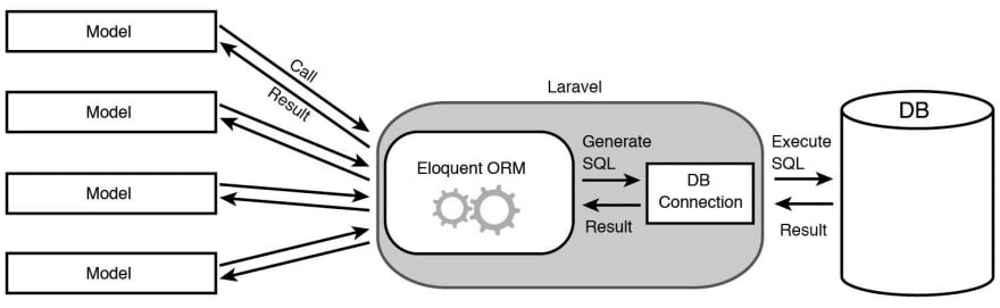
\includegraphics[height=0.2\textheight]{laravel_schema.png}
    \caption[Laravel ORM schema (Eloquent)]{Laravel ORM shema (Eloquent)}
\end{figure}
\subsection{\IfLanguageName{dutch}{Metasploit voor de Laravel-applicatie}{Metasploit for the Laravel application}}
Metasploit is een van de meest uitgebreide security frameworks voor het uitvoeren van penetratietests en 
staat bekend om zijn robuuste exploit-database en modulaire aanpak zoals ik heb vermeld in het hoofdstuk 
\nameref{sec:Webomgevingen} van de literatuurstudie. De Laravel-applicatie, bekend 
om zijn rijke set aan functionaliteiten en complexe architectuur, kan profiteren van Metasploit's 
vermogen om specifieke exploits te gebruiken die zijn afgestemd op gedetecteerde kwetsbaarheden. 
De tool biedt geautomatiseerde exploitatie technieken die essentieel zijn voor het identificeren 
van beveiligingsrisico's in een geavanceerd framework zoals Laravel. Bovendien ondersteunt 
Metasploit de ontwikkeling van aangepaste exploits, wat van grote waarde kan zijn bij 
het testen van functies binnen de te testen Laravel-applicatie.

\subsection{\IfLanguageName{dutch}{Burp Suite voor de wordpress applicatie met beveiligings plugins}{Burp Suite for the wordpress application with security plugins}}
Burp Suite is een geïntegreerd platform voor het testen van de beveiliging van webapplicaties en is 
bijzonder effectief voor het analyseren van HTTP-verkeer en het uitvoeren van geavanceerde web 
aanvallen. Zoals besproken in het hoofdstuk \nameref{sec:Webomgevingen} binnen de literatuurstudie 
biedt Burp Suite uitgebreide functionaliteiten die van belang zijn voor een grondige beveiligingsanalyse 
van webomgevingen. Voor een WordPress-installatie met beveiligingsplugins biedt Burp Suite daarom de noodzakelijke 
diepgang om de effectiviteit van de plugins te evalueren. Door zijn vermogen om verzoeken te 
onderscheppen, te manipuleren en opnieuw te versturen, kunnen testers de robuustheid van 
beveiligingsmaatregelen zoals firewalls en inbraakdetectiesystemen die door plugins worden 
geïmplementeerd, nauwkeurig beoordelen. Burp Suite's scanner, die vervat zit in de enterprise edition kan automatisch een breed scala 
aan kwetsbaarheden identificeren, wat tijd bespaart tijdens de testfase en zorgt voor een 
grondige evaluatie van de beveiligingsstatus.

\subsection{\IfLanguageName{dutch}{OWASP ZAP voor de wordpress applicatie zonder beveiligings plugins}{OWASP ZAP for the wordpress application without security plugins}}
OWASP ZAP (Zed Attack Proxy) is een open-source tool voor het automatisch detecteren van beveiligingsfouten 
in webapplicaties tijdens het ontwikkelings- en testproces. Gezien zijn goede reputatie en uitgebreide 
ondersteuning door de OWASP-community is ZAP bijzonder geschikt voor het testen van een 
WordPress-site zonder aanvullende beveiligingsmaatregelen. ZAP's geïntegreerde scanner en 
intercepting proxy maken het eenvoudig om kwetsbaarheden zoals XSS en SQL-injectie aan te 
tonen, die voorkomen in basisconfiguraties van WordPress. Daarnaast biedt ZAP dynamische 
analyse van de applicatie in real-time, wat helpt bij het direct identificeren van beveiligingsproblemen.


\section{\IfLanguageName{dutch}{Proof of Concept: Gebruiksvriendelijkheid en Effectiviteit van Pentesting Tools voor Webapplicaties}{Proof of Concept: Usability and Effectiveness of Pentesting Tools for Web Applications}}

In de proof of concept testen we de drie verschillende webomgevingen met de vernoemde pentesting tools om hun bruikbaarheid en effectiviteit te evalueren. 
Deze benadering is gericht op het vergelijken van de uitkomsten van pentests in elke omgeving, waardoor kan vastgesteld worden hoe de 
beveiligingsuitdagingen en kwetsbaarheden verschillen.

\subsubsection{\IfLanguageName{dutch}{Omgevingsdiversiteit}{Environmental diversity}}
De aanpak in deze proof of concept is gebaseerd op een realistische benadering, waarbij de drie pentesting tools worden gebruikt die zijn afgestemd 
op de unieke kenmerken van elke omgeving. Het team van Sinergio begrijpt dat geen twee webomgevingen dezelfde zijn en daarom is het belangrijk om een breed scala 
aan tools in te zetten om alle mogelijke kwetsbaarheden en beveiligingsrisico's aan het licht te brengen.

Door deze diversiteit aan tools kan het team niet alleen de specifieke omgeving testen met de best passende tool, maar ook de algehele robuustheid en 
weerbaarheid van de systemen maximaliseren. Elke tool heeft zijn eigen sterke punten en specialiteiten, waardoor een uitgebreide evaluatie mogelijk 
is die verder gaat dan alleen de oppervlakte.

Door te variëren in de gebruikte tools, kan het team verschillende aanvalsscenario's simuleren en de reactie van de systemen daarop beoordelen. Dit 
stelt hen in staat om een diepgaand inzicht te krijgen in de beveiligingsstatus van elke omgeving en biedt waardevolle informatie voor het verbeteren 
van de algehele beveiliging.

\subsubsection{\IfLanguageName{dutch}{Focus van pentesttools}{Focus of the pentesttools}}
De evaluatie van de wordpress beveiligingsplugin wordt geëvalueerd met Burp Suite om op die manier de efficiëntie ervan te testen. De focus ligt op het evalueren van de weerstand 
tegen veelvoorkomende webaanvallen, zoals brute force-aanvallen en SQL-injectie. Ze analyseren hoe de plugin potentiële dreigingen behandelt met 
behulp van Burp Suite en identificeren eventuele tekortkomingen in de bescherming

OWASP ZAP helpt bij het blootleggen van kwetsbaarheden die een website zonder beveiligingsmaatregelen zou kunnen hebben. De nadruk ligt op het 
ontdekken van eenvoudig te exploiteren kwetsbaarheden en het trainen van aan nieuwe gebruikers om deze kwetsbaarheden te begrijpen en 
te leren hoe ze tegen te gaan.

Met Metasploit wordt gefocust op geavanceerdere beveiligingsaspecten, zoals routebescherming en authenticatiemechanismen.
In Laravel is het bijvoorbeeld mogelijk om het aantal mislukte inlogpogingen in te stellen voordat een gebruiker tijdelijk wordt geblokkeerd. Dit wordt vaak gedaan 
als een beveiligingsmaatregel om brute force-aanvallen te voorkomen. Je kunt het aantal inlogpogingen aanpassen door een eigenschap genaamd 
'maxAttempts' in te stellen in de configuratie van het authenticatiesysteem van Laravel. Deze tests zullen 
bijdragen aan het inzicht in de robuustheid van de beveiliging en helpen bij het identificeren van potentieel over het hoofd geziene kwetsbaarheden.

\section{\IfLanguageName{dutch}{Hoe pentesten}{How to pentest}}
Dit hoofdstuk beschrijft de methodologie die wordt gehanteerd voor het uitvoeren van penetratietesten op webapplicaties met behulp van Metasploit, 
Burp Suite Community Edition en OWASP ZAP. De focus ligt hierbij op twee specifieke aanvalstechnieken: brute force-aanvallen en SQL-injecties. 
Het gebruik van deze tools en technieken heeft tot doel inzicht te verkrijgen in de kwetsbaarheden van webapplicaties en de effectiviteit van 
verschillende beveiligingsmaatregelen.

\subsection{\IfLanguageName{dutch}{Voorbereiding van de testomgeving}{Voorbereiding van de testomgeving}}
Voor de uitvoering van de penetratietesten werd een gecontroleerde omgeving opgezet door Sinergio. Deze omgeving omvat een webserver waarop kwetsbare 
applicaties draaien, specifiek ontworpen om te dienen als testdoelen voor beveiligingsanalyses. Hiervoor is de server security via de firewall ook uitgezet zodat 
het IP nooit geblacklist zou worden wanneer een brute-force aanval wordt gesimuleerd. De gebruikte testapplicaties zijn gebaseerd 
op WordPress en Laravel, aangezien deze veelvoorkomende platforms representatief zijn voor echte wereldscenario's.

\subsection{\IfLanguageName{dutch}{Werkwijze metasploit}{Working method metasploit}}
Metasploit kan geïnstalleerd worden op een Windows-systeem. De installatie omvat de nieuwste versie van Metasploit Framework, samen met de 
benodigde updates en dependencies.

\subsubsection{\IfLanguageName{dutch}{Brute-force aanval}{Brute-force attack}}
Om een brute force-aanval uit te voeren met Metasploit op een webapplicatie, wordt gebruikgemaakt van de auxiliary\slash scanner\slash http\slash brute\_dirs
module. Deze module probeert verschillende URL-paden op de webserver te vinden door middel van brute force.
Het te volgen parcours gaat als volgt:
\begin{enumerate}
    \item Start Metasploit en laad de brute\_dirs module
    \begin{enumerate}
        \item msfconsole
        \item use auxiliary\slash scanner\slash http\slash brute\_dirs
    \end{enumerate}
    \item Configureer de module met de doelhost en eventuele andere parameters
    \begin{enumerate}
        \item set RHOSTS (doel-IP)
        \item set THREADS 10
        \item set PATHS (pad-naar-bestand-met-directories)
        \item set PORTS 443\slash 80 
    \end{enumerate}
    \item run
\end{enumerate}
\subsection{\IfLanguageName{dutch}{Werkwijze burp-suite community edition}{Working method  burp-suite community edition}}
Burp Suite Community Edition kan eveneens geïnstalleerd worden op een Windows-systeem. De installatie omvat de configuratie 
van de ingebouwde proxy om het HTTP-verkeer tussen de browser en de webapplicatie te onderscheppen en te analyseren.

\subsubsection{\IfLanguageName{dutch}{Brute-force aanval}{Brute-force attack}}
Met Burp Suite kan een brute force-aanval worden uitgevoerd via de 'Intruder' tool. Hierbij wordt via verschillende wachtwoordcombinaties 
getracht om toegang te verkrijgen tot de webapplicatie. Het proces verloopt als volgt:
\begin{enumerate}
    \item Start Burp Suite en configureer de proxy-instellingen in de browser.
    \item Ga naar de login-pagina van de doelwebapplicatie en onderschep het inlogverzoek met Burp Suite.
    \item Stuur het onderschepte verzoek naar de 'Intruder': Right-click > Send to intruder
    \item Configureer de 'Intruder' met de gewenste payloads (gebruikersnamen en wachtwoorden).
    \item Start de aanval door op 'Start attack' te klikken.
\end{enumerate}

\subsubsection{\IfLanguageName{dutch}{Sql-injection}{Sql-injection}}
Om een SQL-injectieaanval te simuleren wordt gebruikgemaakt van de 'Repeater' tool in Burp Suite. Op de onderstaande manier gemanipuleerde SQL-query's naar de 
server gestuurd.
\begin{enumerate}
    \item Intercept een HTTP-verzoek dat SQL-parameters bevat.
    \item Stuur het onderschepte verzoek naar de 'Repeater': Right-click > Send to repeater
    \item Manipuleer de SQL-parameter in de 'Repeater' en stuur het aangepaste verzoek naar de server.
    \item Analyseer de reactie om te bepalen of de SQL-injectie succesvol was.
\end{enumerate}

\subsection{\IfLanguageName{dutch}{Werkwijze OWASP ZAP}{Working method OWASP ZAP}}
OWASP ZAP kan eveneens geïnstalleerd worden op een Windows-systeem. De installatie omvat het configureren van de ingebouwde 
proxy om het HTTP-verkeer te onderscheppen en te analyseren.
\subsubsection{\IfLanguageName{dutch}{Brute-force aanval}{Brute-force attack}}
OWASP ZAP bevat een ingebouwde tool voor het uitvoeren van brute force-aanvallen op webapplicaties.
De configuratie verloop als volgt:
\begin{enumerate}
    \item Start OWASP ZAP en configureer de proxy-instellingen in de browser.
    \item Ga naar de login-pagina van de doelwebapplicatie en onderschep het inlogverzoek met OWASP ZAP.
    \item Klik met de rechtermuisknop op het onderschepte verzoek en selecteer 'Attack' > 'Forced Browse Site'
    \item Configureer de brute force-instellingen en start de aanval.
\end{enumerate}

\subsubsection{\IfLanguageName{dutch}{Sql-injectie}{Sql-injection}}
Voor een SQL-injectieaanval wordt gebruikgemaakt van de 'Active Scan' feature van OWASP ZAP.
De te nemen stappen zijn daar:
\begin{enumerate}
    \item Intercepteer een HTTP-verzoek dat SQL-parameters bevat.
    \item Voeg het verzoek toe aan de scan queue door met de rechtermuisknop te klikken en 'Attack' > 'Active Scan' te selecteren
    \item Start de actieve scan en analyseer de resultaten om te bepalen of er SQL-injectie kwetsbaarheden zijn.
\end{enumerate}